\newpage
\chapter{Экспериментальные факты, указывающие на существование спина и внутреннего магнитного момента у электрона}
\par Мы познакомились с механическим моментом количества движения. Понятно, что с ним связан магнитный момент. Допустим, знаем токи, как тогда найти момент? По аналогии $\vb{r} \times \vb{j}$, это все идет из уравнений Максвелла: $rot \, \vb{B} = \frac{4 \pi}{c} \vb{j}$, предположим, что можно записать $\vb{j}=c \cdot rot \, \vb{M}$, откуда получим уравнение $rot \left( \vb{B} -4 \pi \vb{M} \right) = rot \, \vb{H} = 0$. Т.о. для нахождения момента по известному току, нужно записать УМ. Есть аналогичная задача - по известному току находится магнитное поле (закон Био-Савара-Лапласа), это и есть $\vb{r} \times \vb{j}$, в этом смысле задача не отличается ничем, кроме констант. Что любопытно: можем установить соотвествие проекции магнитного момента на механический момент (\textbf{гиромагнитное отношение}) для электрона 
$$\frac{M_z}{L_z} =\frac{e}{2mc}$$
\par \begin{remark}  Вычислим силу кругового тока, обусловленного движением электрона по круговой орбите. По определению, сила тока — это количество заряда, протекшего через поперечное сечение за единицу времени. В данном случае электрон за 1 секунду пересечет воображаемое сечение $\nu$ раз, где $\nu$ — частота вращения электрона. Поэтому имеем
$$I = e \nu = e \frac{1}{T} = \frac{e v}{2 \pi r}$$
\par Здесь $T$ - период вращения, а $v$ - линейная скорость электрона. Магнитный момент электрона, обусловленный вращением, равен
$$p_0 = I S = \frac{e}{t}\pi r^2= \frac{e v r}{2}$$
\par Направление вектора $\vb{p_0}$ определяется правилом правого винта. Данный магнитный момент принято называть \textit{орбитальным магнитным моментом электрона}. Движущийся по круговой орбите электрон обладает моментом импульса, который равен:
$$\vb{L_0} = \vb{r} \times m\vb{v}$$
\par Вектор $\vb{L_0}$ направлен противоположно вектору $\vb{p_0}$, а его величина с учетом связи линейной и угловой скоростей движения равна:
$$L_0 = rmv = rmwr = \m \frac{2\pi}{T}r^2 $$
\par Теперь можем найти соотношение, которое называется \textit{гиромагнитным (магнитомеханическим) отношением орбитальных моментов электрона}.
$$\frac{p_0}{L_0} = \frac{e}{2m}$$ 
\par Мы считали, что электрон движется по круговой орбите, но можно показать, что такое же соотношение справедливо и при движении электрона по эллиптической орбите. Гиромагнитное отношение указывает на наличие связи между магнитными и механическими свойствами магнетика. Действительно, если изменились его магнитные свойства, то это должно привести к изменению механических свойств. Справедливо и обратное — изменение механических свойств должно привести к намагничению магнетика. \textbf{Конец замечания.}
\end{remark}
\par Если мы перейдем к квантовой механике, $\vb{L}$ становится оператором $\hat{L}_z$, имеющий некоторый дискретный набор собственных значений, тогда естественно предположить, что с точностью до коэффициента $M_z$ повторяет $L_z$. Отсюда получим дискретные значения магнитного момента. 
\par Для проверки данных соображений в 1921 году Штерном и Герлахом был проведен следующий эксперимент.
\par \begin{wrapfigure}[13]{r}{0.45\linewidth} 
\vspace{-2ex}
\centering
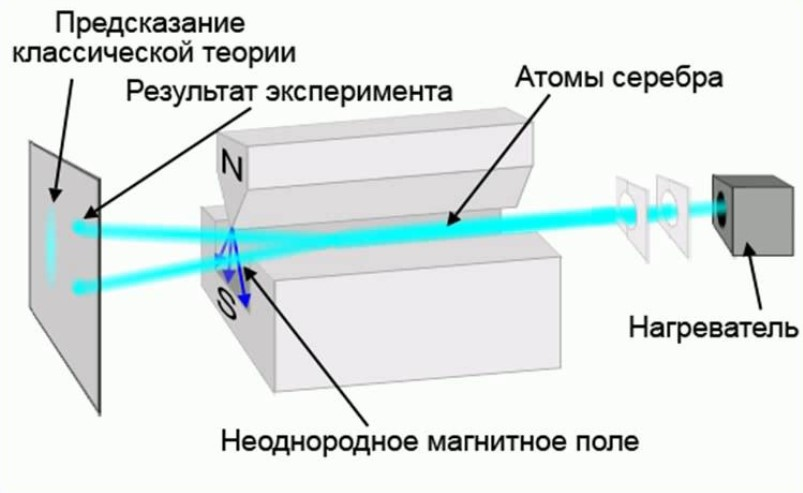
\includegraphics[width=1\linewidth]{pictures/31.1.jpg}
\caption{Опыт Штерна и Герлаха}
\end{wrapfigure}
\par Ставили экран с щелью, посылали на него пучок атома водорода (в оригинале - серебра) в s-состоянии (волновая функция изотропна, \textit{l=0}), далее была область неоднородного магнитного поля и ставили экран. Понятно, что энергия магнитного момента в магнитном поле $U=- \vb{M}\vb{B}$. Если $\vb{B}$ неоднородно, а $\vb{M}$ квантовано, то градиент потенциальной энергии даст силу, которая по-разному будет отклонять атомы, что даст какие-то дискретные следы на экране. В опыте получались 2 резких линии. Если бы это были классические частицы, мы бы получили некоторый разброс, но эта линия была бы одна и размытая. Вообще мы рассматриваем s-состояние, где нет орбитального и магнитного момента, о какой линии тогда может идти речь? Может, прогадали с условиями эксперимента, смотрим дальше: число проекций магнитного момента всегда нечетное (!), а получается явно две (!) полоски. Это был один из важных сигналов: волновая механика электрона в своей первоначальной форме не позволяет объяснить некоторых фактов магнитных и спектроскопических (см. далее) измерений.

\par Второй звоночек. В натрии изучали переход состоянии из $2p$ в $1s$ (первое число - это главное квантовое, s и p - квантовые). Увидели так называемый \textit{дублет} - две близкие линии. Опять возвращаемся к уже полученному противоречию. 
\par \begin{wrapfigure}[9]{l}{0.45\linewidth} 
\vspace{-2ex}
\centering
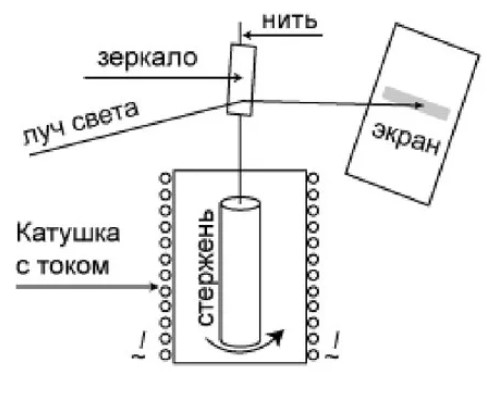
\includegraphics[width=0.7\linewidth]{pictures/31.2.jpg}
\caption{Опыт Эйнштейна-де-Гааза}
\end{wrapfigure}
\par Еще ранее, в 1915 году, был проведен еще один эксперимент - опыт Эйнштейна и Де Гааза

\par Тонкий железный стержень (ферромагнитный цилиндр) подвешивался на упругой нити и помещался внутрь соленоида. Для усиления эффекта применен метод резонанса - по соленоиду протекал переменный ток, частота которого подбиралась равной собственой частоте механических колебаний стержня. При намагничивании стержня магнитные моменты электронов установятся по направлению поля, а механические моменты против поля. В результате суммарный момент импульса электронов станет отличен от нуля. Момент импульса системы (стержень + электроны) должен остаться неизменным, поэтому стержень начнет закручиваться против вращения электронов. По измеренной амплитуде колебаний можно вычислить и механический момент, и гиромагнитное отношение, которое оказалось равным:
$$\frac{p_0}{L_0} = \frac{e}{m}$$
\par Отличие в 2 раза напрягало людей. В 1925 году Уленбек и Гоудсмит предположили, что у электрона, помимо того самого орбитального момента, который есть $\hbar m_z$, существует еще свой, \textbf{внутренний момент} - $S_z= \pm \hbar / 2$ и магнитный момент, который удовлетворяет гиромагнитному отношению без двойки. Проблема "полуцелых" состояний: выполнено условие невыделенности направления оси M (допустимые состояния -1/2 и 1/2), но волновая функция  $\psi$ этих состояний при повороте на $2\pi$ меняет знак, что на самом деле несколько тревожно. С другой стороны, нас интересует $|\psi|^2$, поэтому пока не будем обращать внимание на этот момент, посмотрим, что выйдет. Так появился \textbf{спин} - внутренний механический момент частицы.
\par Для спина собственных значений оператора $\hat{S}^2$ всего $s(s+1)$, для электрона $s=1/2$. Как ввести оператор спина - об этом и о других интересных фактах из жизни электрона смотри в следующем семестре.